\documentclass[24pt,pdf,hyperref={unicode}]{beamer}
\usepackage[utf8]{inputenc}
\usepackage{aiml}
\begin{document}


\section{Дедуктивные и индуктивные рассуждения}

\begin{frame}\frametitle{Индуктивные рассуждения}
\begin{tabular}{l l}
 & Бразилия -- страна Южной Америки и республика \\
 & Чили -- страна Южной Америки и республика \\
 & Уругвай -- страна Южной Америки и республика \\
\hline
$\therefore$ & Все страны Южной Америки -- республики \\
\end{tabular}
\end{frame}

\begin{frame}\frametitle{Индуктивные рассуждения}
\begin{tabular}{l l}
 & Франция -- страна Европы и республика \\
 & Германия -- страна Европы и республика \\
 & Чехия -- страна Европы и республика \\
\hline
$\therefore$ & Все страны Европы -- республики \\
\end{tabular}
\begin{flushright}
% \uncover{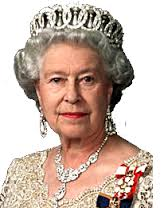
\includegraphics[width=4cm]{EnglishQueen.jpg}}
\end{flushright}
\end{frame}


\begin{frame}\frametitle{Индуктивные рассуждения}
\begin{tabular}{l l}
 & Бразилия -- республика и страна Южной Америки \\
 & Чили -- республика и страна Южной Америки \\
 & Уругвай -- республика и страна Южной Америки \\
\hline
$\therefore$ & Все республики -- страны Южной Америки\\
\end{tabular}
\begin{flushright}
% \uncover{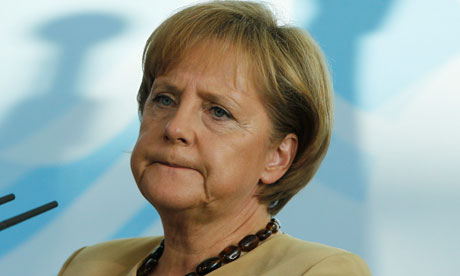
\includegraphics[width=4cm]{Merkel.jpg}}
\end{flushright}
\end{frame}


\begin{frame}\frametitle{Дедуктивные рассуждения}
\begin{tabular}{l l}
 & Все страны Южной Америки -- республики \\
 & Бразилия -- страна Южной Америки\\
 \hline
$\therefore$ & Бразилия -- республика \\
\end{tabular}
\end{frame}

\begin{frame}\frametitle{Дедуктивные рассуждения}
\begin{tabular}{l l}
 & Все моря -- соленые \\
 & Черное море -- это море \\
 \hline
$\therefore$ & Черное море -- соленое \\
\end{tabular}
\end{frame}

\begin{frame}\frametitle{Дедуктивные рассуждения}
\begin{tabular}{l l}
 & Все $A$ есть $B$\\
 & Некоторый $x$ является $B$\\
 \hline
$\therefore$ & $x$ является $A$ \\
\end{tabular}
\end{frame}

\section{Пропозициональная логика}

\begin{frame}\frametitle{Пропозициональные связки }
Не очень понятно, как здесь сделать нормальную анимацию
\end{frame}

\section{Логический вывод}

\begin{frame}\frametitle{Modus ponens}
{\huge
$$
\frac{A,\ A\rightarrow B}{B}
$$
}
\end{frame}

\begin{frame}\frametitle{Аксиомы}
\begin{enumerate}
 \item[A1] $A\rightarrow(B\rightarrow A)$
 \item[A2] $\left[A\rightarrow(B\rightarrow C)\right]\rightarrow\left[(A\rightarrow B)\rightarrow(A\rightarrow C)\right]$
 \item[A3] $(\neg A\rightarrow \neg B)\rightarrow\left[(\neg A\rightarrow B)\rightarrow A\right]$
\end{enumerate}
\end{frame}

\begin{frame}\frametitle{$X\rightarrow X$?}
$$
\begin{array}{l l}
\uncover<+->{A2 & \left[A\rightarrow(B\rightarrow C)\right]\rightarrow\left[(A\rightarrow B)\rightarrow(A\rightarrow C)\right]}\\
\uncover<+->{& A=X,\ B=X\rightarrow X,\ C=X}\\
\uncover<+->{L1 & \left[X\rightarrow((X\rightarrow X)\rightarrow X)\right]\rightarrow\left[(X\rightarrow (X\rightarrow X))\rightarrow(X\rightarrow X)\right]}\\
\uncover<+->{A1 & A\rightarrow(B\rightarrow A)} \\
\uncover<+->{& A=X,\ B=X\rightarrow X}\\
\uncover<+->{L2 & X\rightarrow((X\rightarrow X) \rightarrow X)} \\
\uncover<+->{MP & (X\rightarrow (X\rightarrow X))\rightarrow(X\rightarrow X)} \\
\uncover<+->{A1 & A\rightarrow(B\rightarrow A)} \\
\uncover<+->{& A=X,\ B=X}\\
\uncover<+->{L3 & X\rightarrow (X\rightarrow X)} \\
\uncover<+->{MP & X\rightarrow X}
\end{array}
$$

\end{frame}





\section{Законы логики высказываний}
\begin{frame}\frametitle{Законы логики высказываний}
\begin{tabular}{l l p{1cm} l}
\multirow{2}{*}{Операции с константами} & $A\vee 0 = A$ && $A\wedge 0=0$ \\
					& $A\vee 1 = 1$ && $A\wedge 1=A$ \\ 		
Идемпотентность & $A\vee A = A$ && $A \wedge A = A$ \\
Ассоциативность & $\begin{array}{l l}
		    A\vee (B\vee C) & = \\
		    (A\vee B)\vee C & = \\
		    A\vee B\vee C
		    \end{array}$
				     &&
					$\begin{array}{l l}
					  A\wedge (B\wedge C) & = \\
					  (A\wedge B)\wedge C & = \\
					  A\wedge B\wedge C
					  \end{array}$ \\
							 
\end{tabular}
\end{frame}

\begin{frame}\frametitle{Конъюнктивная нормальная форма}

$$
\begin{array}{l l l}
& (A \vee B \vee C) & \wedge \\
& (\neg A \vee B \vee \neg C) & \wedge \\
& (\neg A)
\end{array}
$$
\end{frame}

\begin{frame}\frametitle{Конъюнктивная нормальная форма}
$$
\begin{array}{l}
\uncover<+->{ \neg A } \\
\uncover<+->{ \neg A \vee B } \\
\uncover<+->{ (A \vee B) \vee C } \uncover<+->{ = A\vee B\vee C }\\
\uncover<+->{ (A \wedge B) \vee C } \uncover<+->{ = (A\vee C)\wedge (B\vee C)}\\
\end{array}
$$
\end{frame}

\begin{frame}\frametitle{Приведение к КНФ}
$$
\begin{array}{l}
\neg A\rightarrow \overline{B\rightarrow C} \\
\uncover<+->{ A \vee \overline{\neg B \vee C }} \\
\uncover<+->{ A \vee (B \wedge \neg C) } \\
\uncover<+->{ (A\vee B) \wedge (A \vee \neg C) }
\end{array}
$$
\end{frame}

\section{Метод резолюций}

\begin{frame}\frametitle{Правило резолюций}
{\huge
$$
\frac{A\vee B,\ \neg A \vee C}{B \vee C}
$$
}
\end{frame}

\begin{frame}\frametitle{Правило резолюций}
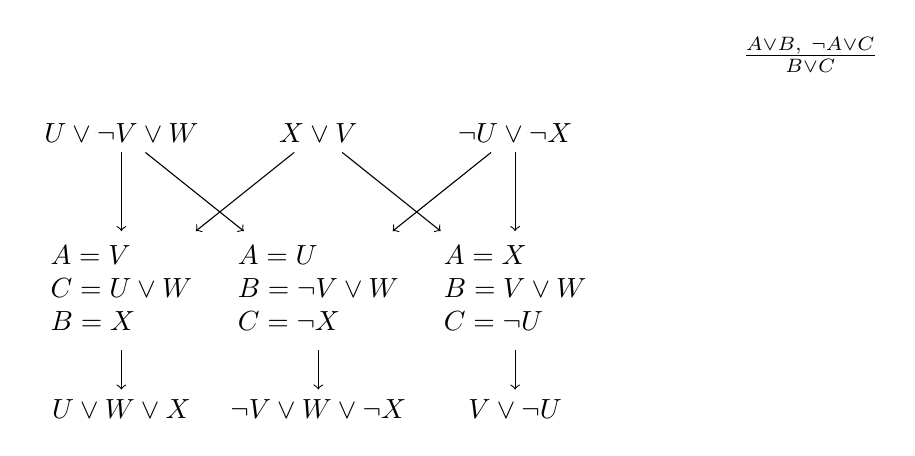
\begin{tikzpicture}[x=2.5cm]
\node at (3.5,4) {$\frac{A\vee B,\ \neg A \vee C}{B \vee C}$};
\node (p1) at (0,3) {$U\vee \neg V \vee W$};
\node (p2) at (1,3) {$X\vee V$};
\node (p3) at (2,3) {$ \neg U\vee \neg X$};

\uncover<2->{
\node (s1) at (0,1) {$\begin{array}{l} A=V\\ C=U\vee W\\ B=X \end{array}$};
\node (r1) at (0,-0.5) {$U\vee W\vee X$};
\path (p1) edge[->] (s1);
\path (p2) edge[->] (s1);
\path (s1) edge[->] (r1);
}

\uncover<3->{
\node (s2) at (1,1) {$\begin{array}{l} A=U\\ B=\neg V \vee W\\ C=\neg X \end{array}$};
\node (r2) at (1,-0.5) {$\neg V\vee W\vee \neg X$};
\path (p1) edge[->] (s2);
\path (p3) edge[->] (s2);
\path (s2) edge[->] (r2);
}

\uncover<4->{
\node (s3) at (2,1) {$\begin{array}{l} A=X\\ B=V \vee W\\ C=\neg U \end{array}$};
\node (r3) at (2,-0.5) {$V\vee \neg U$};
\path (p2) edge[->] (s3);
\path (p3) edge[->] (s3);
\path (s3) edge[->] (r3);
}
\end{tikzpicture}
\end{frame}

\begin{frame}\frametitle{Правило резолюций}
\begin{tikzpicture}[x=2.2cm]
\node at (4,4) {$\frac{A\vee B,\ \neg A \vee C}{B \vee C}$};
\node (p2) at (0,3) {$X$};
\node (p1) at (1.5,3) {$\neg X \vee Y \vee Z$};
\node (p3) at (3,3) {$\neg Z$};

\uncover<2->{
\node at (4,3) {$\frac{A\rightarrow B,\ A}{B}$};

\node (t1) at (0.75,2) {$X\rightarrow Y\vee Z$};
\node (s1) at (0.5,0.5) {$\begin{array}{l} A=X\\ B=Y\vee Z\end{array}$};
\node (r1) at (0.5,-1) {$Y\vee Z$};

\path (p1) edge[->] (t1);
\path (t1) edge[->] (s1);
\path (p2) edge[->] (s1);
\path (s1) edge[->] (r1);
}

\uncover<3->{
\node (t2) at (2.25,2) {$\neg Z\rightarrow \neg X\vee Y$};
\node (s2) at (2.5,0.5) {$\begin{array}{l} A=\neg Z\\ B=\neg X \vee Y\end{array}$};
\node (r2) at (2.5,-1) {$\neg X \vee Y$};

\path (p1) edge[->] (t2);
\path (t2) edge[->] (s2);
\path (p3) edge[->] (s2);
\path (s2) edge[->] (r2);
}

\end{tikzpicture}
\end{frame}

\begin{frame}\frametitle{Правило резолюций}
\begin{tikzpicture}[x=2.5cm]
\node at (3.5,4) {$\frac{A\vee B,\ \neg A \vee C}{B \vee C}$};
\node (p1) at (0,3) {$\neg X \vee U \vee V$};
\node (p2) at (1,3) {$X$};
\node (p3) at (2,3) {$\neg X$};

\node (s1) at (0.5,1) {$\begin{array}{l} A=X\\ B=\square \\ C= U \vee V \end{array}$};
\node (r1) at (0.5,-0.5) {$U\vee V$};
\path (p1) edge[->] (s1);
\path (p2) edge[->] (s1);
\path (s1) edge[->] (r1);

\node (s2) at (1.5,1) {$\begin{array}{l} A=X\\ B=\square \\ C= \square\end{array}$};
\node (r2) at (1.5,-0.5) {$\square$};
\path (p2) edge[->] (s2);
\path (p3) edge[->] (s2);
\path (s2) edge[->] (r2);
\end{tikzpicture}
\end{frame}

\begin{frame}\frametitle{Правило резолюций}
\begin{tikzpicture}[x=2.5cm]
\node (p1) at (0,3) {$\neg X \vee \neg Y \vee U$};
\node (p2) at (1,3) {$X \vee Y \vee V$};

\only<2>
{
\path (p1) edge[->] (r1);
\path (p2) edge[->] (r1);
\node (r1) at (0.5,-0.5) {$U\vee V$};
}

\only<3-4>
{
\node at (3,4) {$\frac{A\vee B,\ \neg A \vee C}{B \vee C}$};
\node (s1) at (0.5,1) {$\begin{array}{l} A=X\vee Y\\ B=V\\ C=U \end{array}$};
\path (p1) edge[->] (s1);
\path (p2) edge[->] (s1);
}

\only<4>
{
\node  at (0.5,-0.5) {$\begin{array}{l} \neg A=\neg X\vee \neg Y \\ \neg A=\neg(X\vee Y)=\neg X\wedge \neg Y\end{array}$};
}

\only<5-6>
{
\node (s1) at (0.5,1) {$\begin{array}{l} A=X\\ B=Y \vee V\\ C=\neg Y \vee U\end{array}$};
\path (p1) edge[->] (s1);
\path (p2) edge[->] (s1);
}

\only<6>
{
\node (r2) at (0.5,-0.5) {$Y\vee V\vee \neg Y \vee U = 1$};
\path (s1) edge[->] (r2);
}

\end{tikzpicture}
\end{frame}

\begin{frame}\frametitle{Метод резолюций}
\uncover<+->{
{\bf Доказать:} 
$$
A_1,A_2,\ldots,A_n\models B
$$
}

\uncover<+->{
{\bf Эквивалентно:} 
$$
A_1,A_2,\ldots,A_n, \neg B\models \square
$$
}

\uncover<+->{
{\bf Алгоритм:}
\begin{enumerate}
\item Привести $A_1,A_2,\ldots,A_n, \neg B$ в КНФ
\item Применять правило резолюций, пока не получится пустая дизъюнкция
\end{enumerate}
} 
\end{frame}

\begin{frame}\frametitle{Метод резолюций}
Сюда пример
\end{frame}

\end{document}
